\begin{figure}[H]
	\centering
	%\begin{subfigure}[b]
		%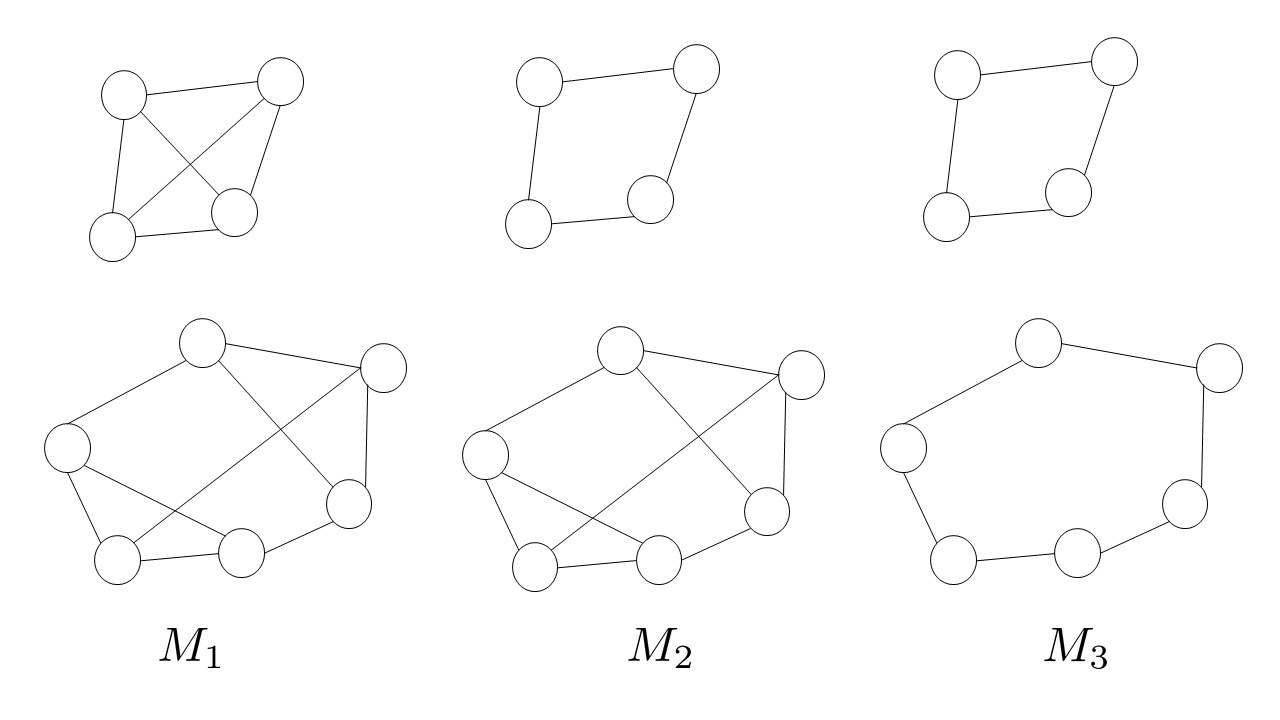
\includegraphics[scale=0.16]{diagrams/example1.jpg}
		%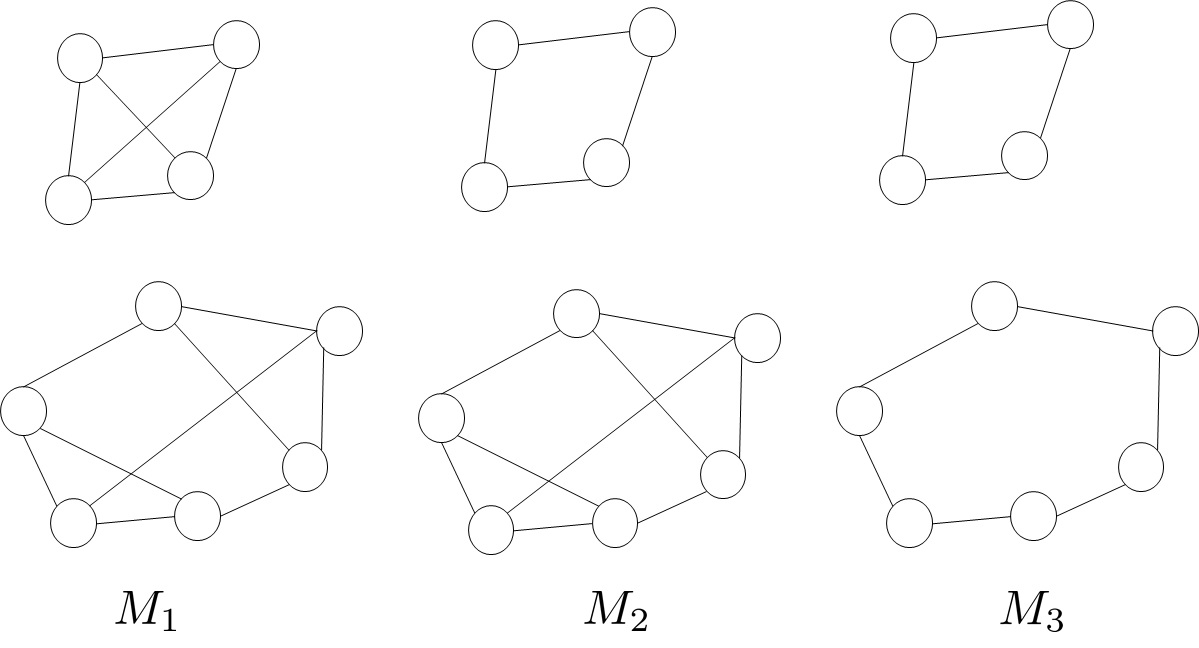
\includegraphics[width=\textwidth]{diagrams/Example_1.png}
		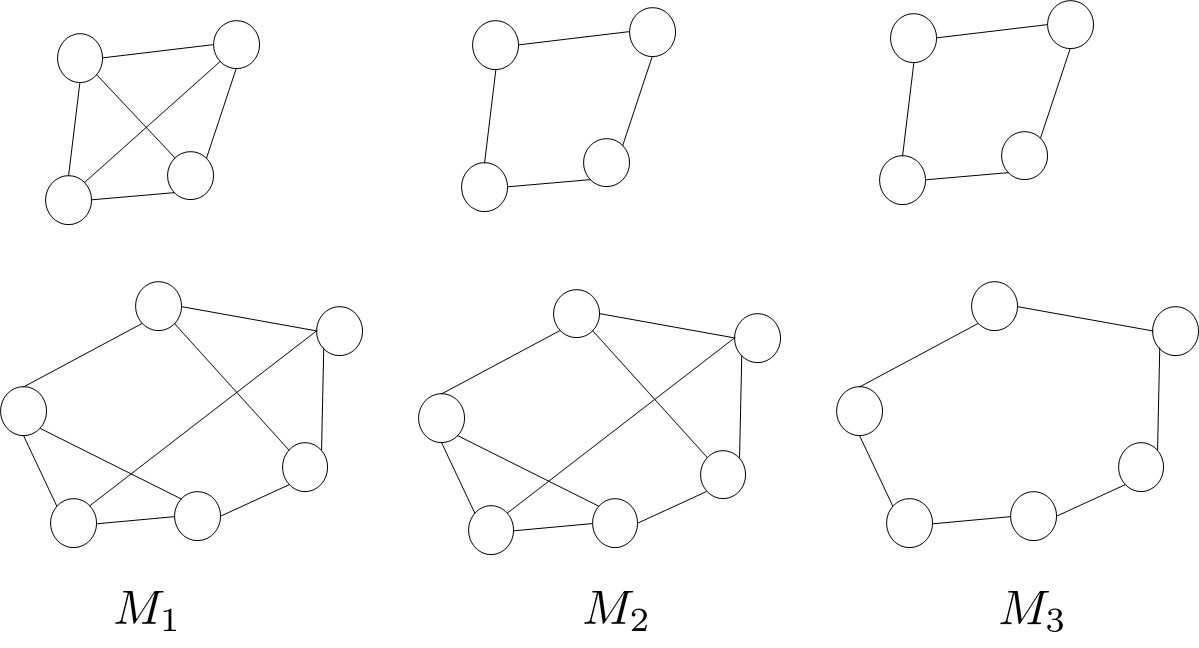
\includegraphics[width=0.7\textwidth]{Ex1.png}
		\caption{$\dist{M_1}{M_2}=1-\specr{\srprod{M_1}{M_2}}$ is not a metric. $\dist{M_1}{M_2}=\dist{M_2}{M_3}=0,$ but 
			$\dist{M_1}{M_3}> 0$.}
		\vspace{3ex}
		\label{fig:example1}
	%\end{subfigure}
	
	%\begin{subfigure}[b]{4.95cm}
		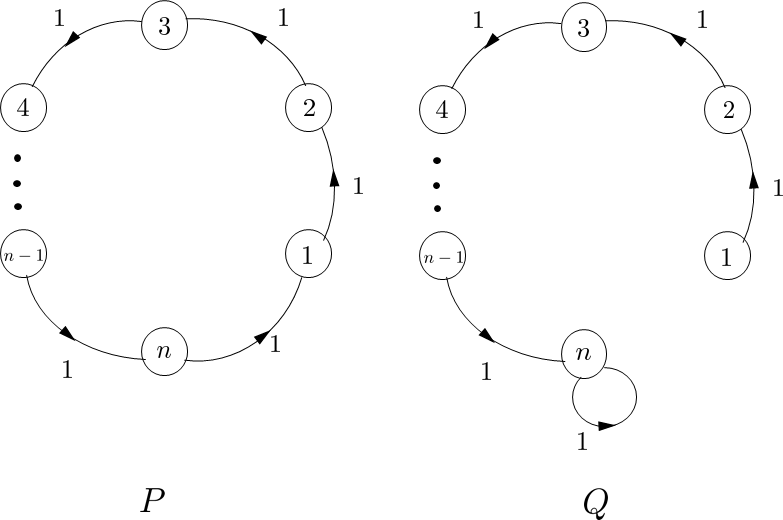
\includegraphics[width=0.5\textwidth]{Ex2.png}
		\caption{To distinguish $P$ vs. $Q$ walking from a random state we need $\Omega(n)$ steps, but $\dist{P}{Q}=1$.}
		\label{fig:example2}
	%\end{subfigure}
	\hspace{3pt}
\end{figure}

\begin{figure}[H]
\centering
	%\begin{subfigure}[b]{4.95cm}
		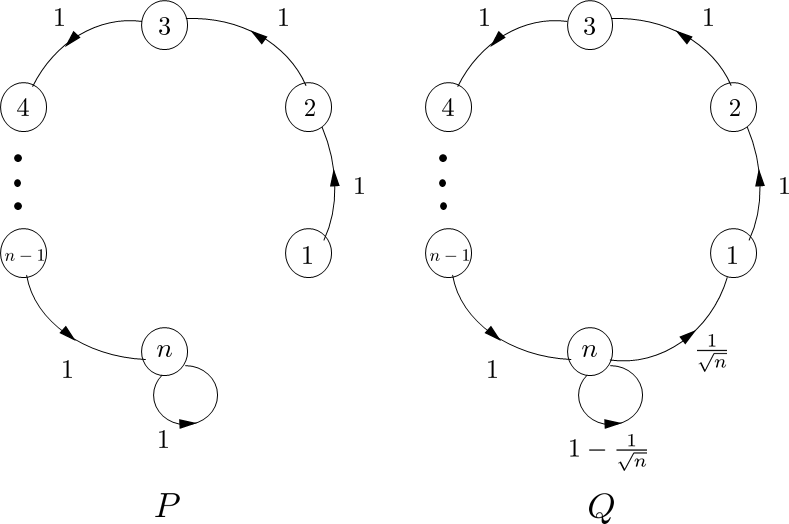
\includegraphics[width=0.5\textwidth]{Ex3.png}
		\caption{$\dist{P}{Q}=o(1)$, stationary distributions $\vect{q}_0,\vect{p}_0$ 
			are different: $\dtv{\vect{q}_0}{\vect{p}_0}=1-o(1)$.}
		\label{fig:example3}
	%\end{subfigure}
	\hspace{3pt}
	%\begin{subfigure}[b]{4.95cm}
		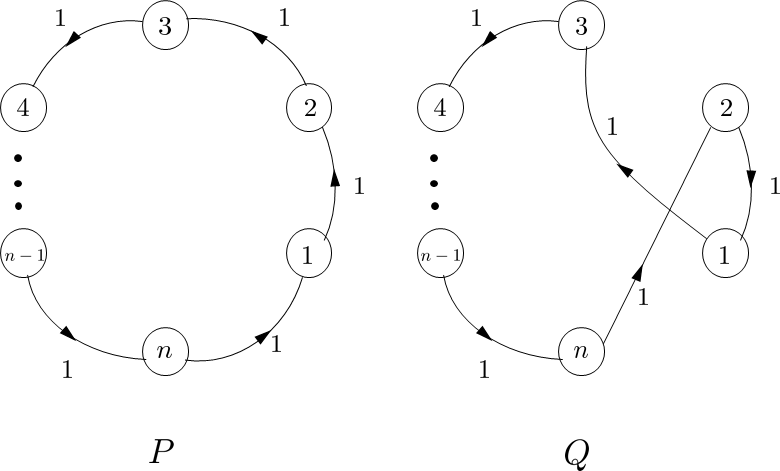
\includegraphics[width=0.5\textwidth]{Ex4.png}
		\caption{$\dist{P}{Q}=1$. Uniform is stationary	for both $P$ and $Q$. 
			On average $\Omega(n)$ steps to tell $P\neq Q$.}
		\label{fig:example4}
	%\end{subfigure}
	
	\hspace{5pt}	
	%\begin{subfigure}[b]{7cm}
		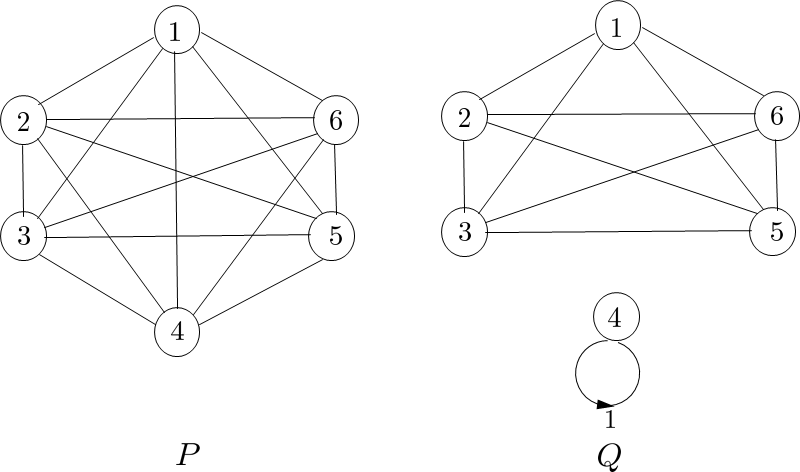
\includegraphics[width=0.7\textwidth]{Ex5.png}
		\caption{After one step from state $4$, we would know if $w\sim P$, or $w\sim Q$. 
			If $w$ starts from any other state $s_0\neq 4$, it would take many steps.}
		\vspace{3ex}
		\label{fig:example5}
	%\end{subfigure}
\end{figure}
	
	
	\vspace{5ex}
	\begin{table}
	\begin{tabular}{ | l | p{0.8\textwidth} |}
		\cline{2-2}
		%\multicolumn{1}{|c|}{Description}
		
		\multicolumn{1}{c|}{} &  \multicolumn{1}{c|}{Description} \\ \hline
		Example~\ref*{fig:example1} & Two disjoint connected components. \\ \hline
		Example~\ref*{fig:example5} & $Q$ -- clique $K_n$; $P$ -- clique $K_{n-1}$ and disjoint vertex.
		Eigenvalue of $\srprod{P}{Q}$: $\eigi[1]=\sqrt{\frac{n-1}{n}}=1-o(1)$, 
		$\eigi[2]=\sqrt{\frac{1}{n}}$, $\eigi[3]=\cdots=\eigi[n]=0$	\\  \hline												
		Example~\ref*{fig:example2} & $P$ -- oriented cycle, $Q$ -- cycle with one link substituted by a loop.\\ \hline
		Example~\ref*{fig:example3} & $P$ -- oriented cycle with edge $e=(v_1v_2)$ substituted by a loop at $v_1$; 
		$Q$ is almost like $P$, but $e$ has weight $\frac{1}{\sqrt{n}}$, loop at $v_n$ has weight $1-\frac{1}{\sqrt{n}}$. 
		Stationary distributions: $\vect{p}_0=\trans{(1,0,\cdots,0)}$ 
		and $\vect{q}_0=\trans{(\frac{\sqrt{n}}{n+\sqrt{n}-1},\frac{1}{n+\sqrt{n}-1},\dots,\frac{1}{n+\sqrt{n}-1})}$. 
		$\specr{\srprod{P}{Q}}=\sqrt{1-\frac{1}{\sqrt{n}}}$.   \\  \hline
		Example~\ref*{fig:example4} & Two oriented cycles $P\eqdef s_1\to s_2\to\cdots\to s_n\to s_1$ and 
		$Q\eqdef s_1\to s_3\to s_4\cdots\to s_n\to s_2\to s_1$.	\\  \hline											
	\end{tabular}
	\caption{Examples.} \label{fig:examples}
	\end{table}


%\begin{figure}[H]
	%\floatconts
	%\subfigure[b]{
		%%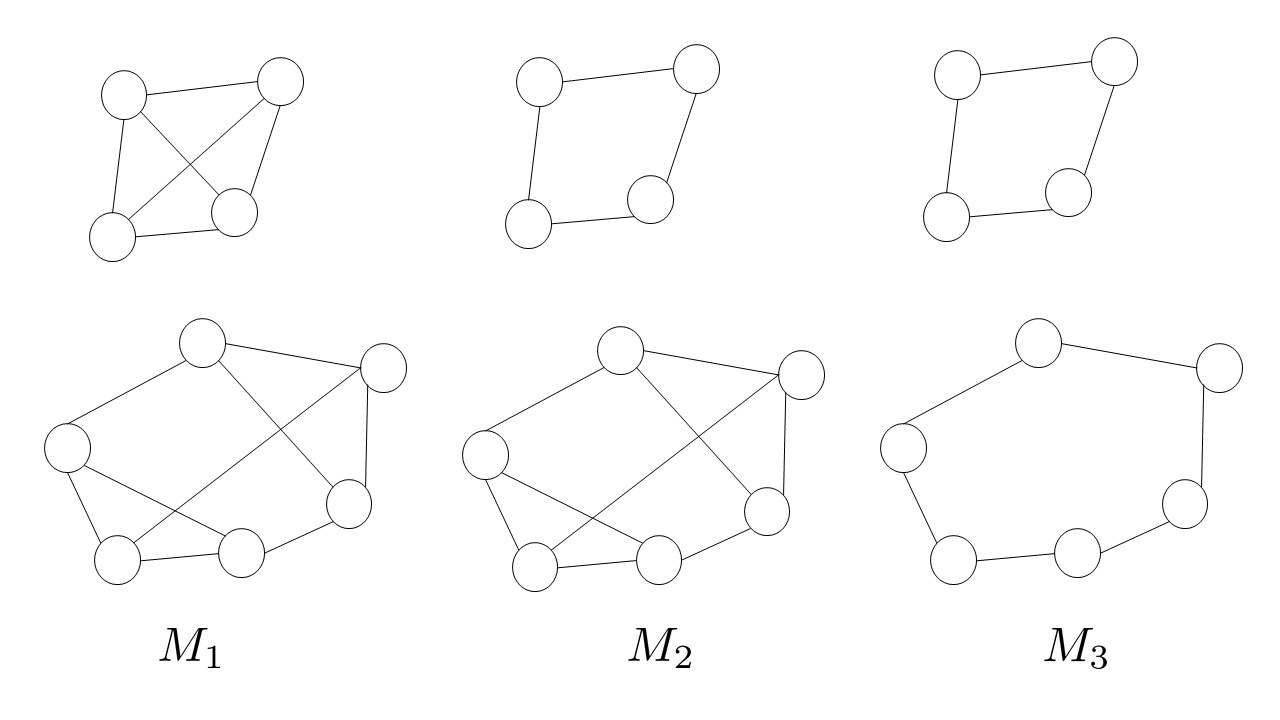
\includegraphics[scale=0.16]{diagrams/example1.jpg}
		%%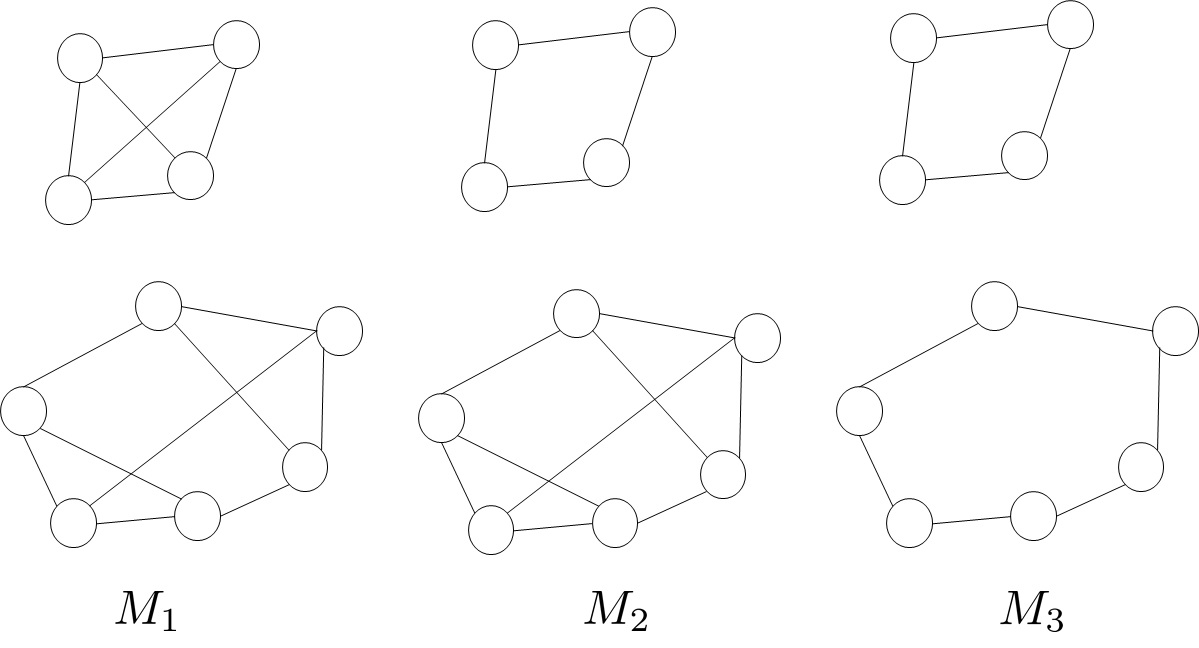
\includegraphics[width=\textwidth]{diagrams/Example_1.png}
		%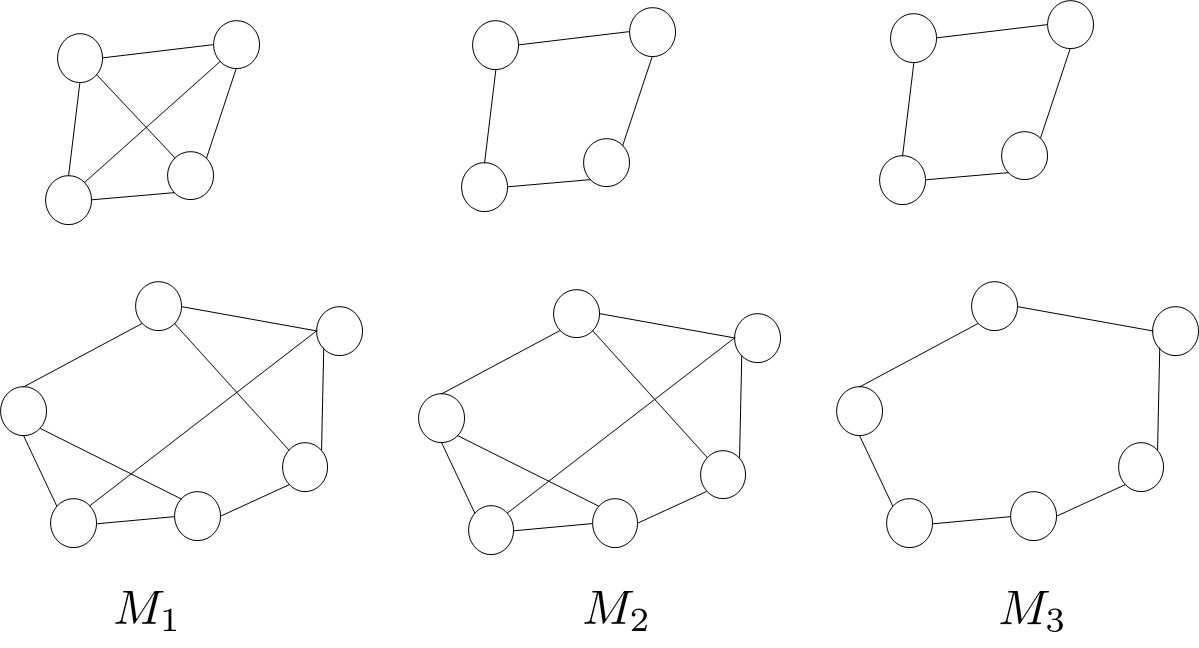
\includegraphics[width=7.45cm]{Ex1.png}
		%\caption{$\dist{M_1}{M_2}=1-\specr{\srprod{M_1}{M_2}}$ is not a metric. $\dist{M_1}{M_2}=\dist{M_2}{M_3}=0,$ but 
			%$\dist{M_1}{M_3}> 0$.}
		%\vspace{3ex}
		%\label{fig:example1}
	%}
	%%\end{subfigure}
	%\hspace{5pt}
	%\floatconts	
	%\subfigure[b]{
		%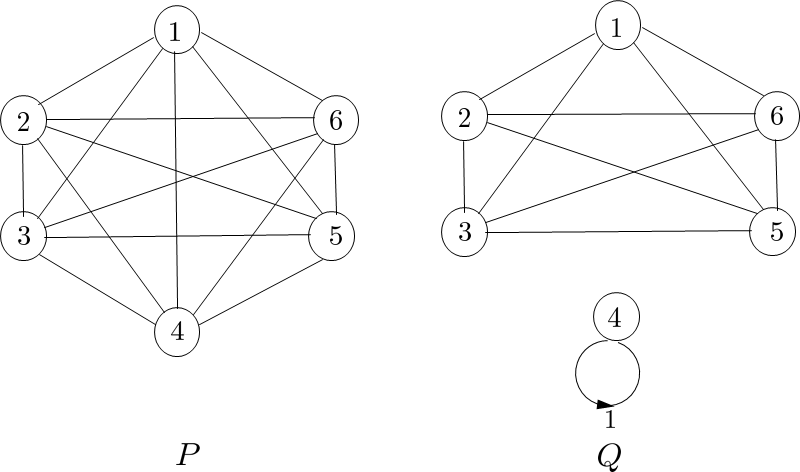
\includegraphics[width=0.45\textwidth]{Ex5.png}
		%\caption{After one step from state $4$, we would know if $w\sim P$, or $w\sim Q$. 
			%If $w$ starts from any other state $s_0\neq 4$, it would take many steps.}
		%\vspace{3ex}
		%\label{fig:example5}
	%}
	%%\end{subfigure}
	%\floatconts
	%\subfigure[b]{
		%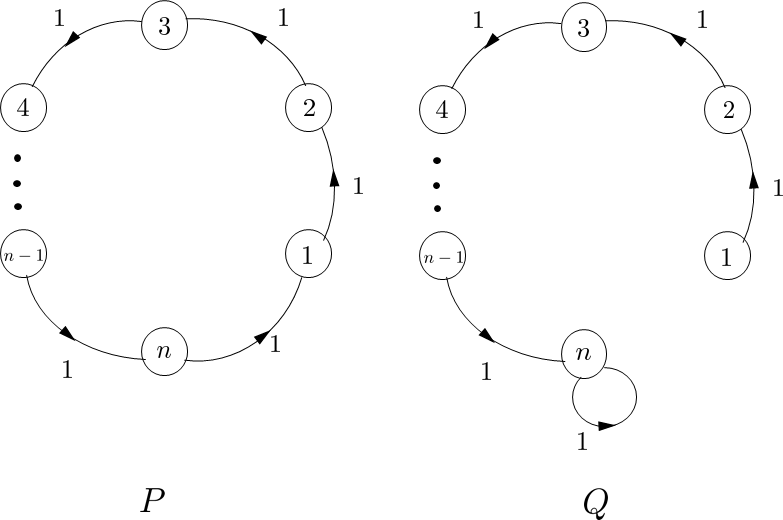
\includegraphics[width=0.9\textwidth]{Ex2.png}
		%\caption{To distinguish $P$ vs. $Q$ walking from a random state we need $\Omega(n)$ steps, but $\dist{P}{Q}=1$.}
		%\label{fig:example2}
	%}
	%%\end{subfigure}
	%\hspace{3pt}
	%\floatconts	
	%\subfigure[b]{
		%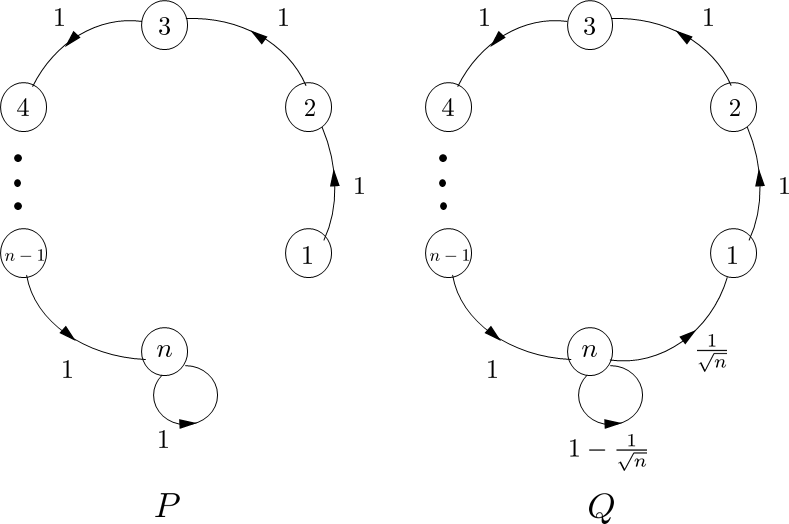
\includegraphics[width=0.9\textwidth]{Ex3.png}
		%\caption{$\dist{P}{Q}=o(1)$, stationary distributions $\vect{q}_0,\vect{p}_0$ 
			%are different: $\dtv{\vect{q}_0}{\vect{p}_0}=1-o(1)$.}
		%\label{fig:example3}
	%}
	%%\end{subfigure}
	%\hspace{3pt}
	%\floatconts
	%\subfigure[b]{
		%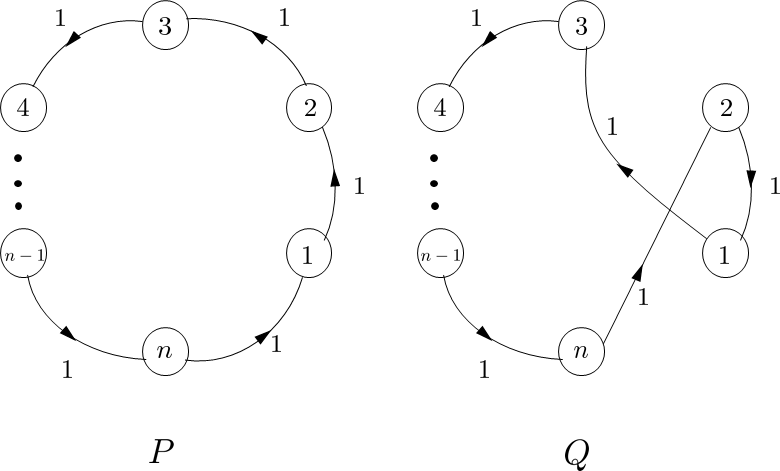
\includegraphics[width=0.9\textwidth]{Ex4.png}
		%\caption{$\dist{P}{Q}=1$. Uniform is stationary	for both $P$ and $Q$. 
			%On average $\Omega(n)$ steps to tell $P\neq Q$.}
		%\label{fig:example4}
	%}
	%%\end{subfigure}
	%
	%\vspace{5ex}
	%\begin{tabular}{ | l | p{0.8\textwidth} |}
		%\cline{2-2}
		%%\multicolumn{1}{|c|}{Description}
		%
		%\multicolumn{1}{c|}{} &  \multicolumn{1}{c|}{Description} \\ \hline
		%Example~\ref*{fig:example1} & Two disjoint connected components. \\ \hline
		%Example~\ref*{fig:example5} & $Q$ -- clique $K_n$; $P$ -- clique $K_{n-1}$ and disjoint vertex.
		%Eigenvalue of $\srprod{P}{Q}$: $\eigi[1]=\sqrt{\frac{n-1}{n}}=1-o(1)$, 
		%$\eigi[2]=\sqrt{\frac{1}{n}}$, $\eigi[3]=\cdots=\eigi[n]=0$	\\  \hline												
		%Example~\ref*{fig:example2} & $P$ -- oriented cycle, $Q$ -- cycle with one link substituted by a loop.\\ \hline
		%Example~\ref*{fig:example3} & $P$ -- oriented cycle with edge $e=(v_1v_2)$ substituted by a loop at $v_1$; 
		%$Q$ is almost like $P$, but $e$ has weight $\frac{1}{\sqrt{n}}$, loop at $v_n$ has weight $1-\frac{1}{\sqrt{n}}$. 
		%Stationary distributions: $\vect{p}_0=\trans{(1,0,\cdots,0)}$ 
		%and $\vect{q}_0=\trans{(\frac{\sqrt{n}}{n+\sqrt{n}-1},\frac{1}{n+\sqrt{n}-1},\dots,\frac{1}{n+\sqrt{n}-1})}$. 
		%$\specr{\srprod{P}{Q}}=\sqrt{1-\frac{1}{\sqrt{n}}}$.   \\  \hline
		%Example~\ref*{fig:example4} & Two oriented cycles $P\eqdef s_1\to s_2\to\cdots\to s_n\to s_1$ and 
		%$Q\eqdef s_1\to s_3\to s_4\cdots\to s_n\to s_2\to s_1$.	\\  \hline											
	%\end{tabular}
	%
	%\caption{Examples.} \label{fig:examples}
%\end{figure}